\documentclass[10pt,twocolumn]{article}

\usepackage[a4paper,top=17mm,bottom=19mm,left=16mm,right=16mm,columnsep=7mm]{geometry}
\usepackage[T1]{fontenc}
\usepackage{newtxtext,newtxmath}
\usepackage{microtype}
\usepackage{graphicx}
\usepackage{booktabs}
\usepackage{array}
\usepackage{amsmath}
\usepackage{siunitx}
\usepackage{xcolor}
\usepackage{caption}
\usepackage{subcaption}
\usepackage{cuted}
\usepackage{tikz}
\usetikzlibrary{arrows.meta,positioning,fit,calc}
\usepackage[numbers,sort&compress]{natbib}
\renewcommand{\bibfont}{\footnotesize}
\setlength{\bibsep}{1.5pt plus 0.5pt}
\usepackage[colorlinks=true,allcolors=blue!55!black]{hyperref}

\definecolor{YouthBlue}{HTML}{1F77B4}
\definecolor{IdentityTeal}{HTML}{2A9D8F}
\definecolor{SOKMRed}{HTML}{C94C4C}
\definecolor{SoftGray}{HTML}{F1F3F5}
\definecolor{TextGray}{HTML}{4D5156}

\graphicspath{{figures/}}
\captionsetup{font=footnotesize,labelfont=bf,justification=justified,singlelinecheck=false}
\setlength{\parindent}{1em}
\setlength{\parskip}{0pt}
\setlength{\textfloatsep}{8pt plus 2pt minus 2pt}
\setlength{\floatsep}{7pt plus 2pt minus 2pt}
\setlength{\intextsep}{7pt plus 2pt minus 2pt}
\setlength{\stripsep}{6pt plus 1pt minus 1pt}
\sisetup{detect-all,round-mode=places,round-precision=4}

\newcommand{\YouthScore}{\textit{Youth Score}}
\newcommand{\IdentityScore}{\textit{Identity Score}}
\newcommand{\SOKM}{SOKM}

\begin{document}
\raggedbottom

\twocolumn[
\begin{@twocolumnfalse}
\begin{center}
{\LARGE\bfseries My Youth Score and MSC Identity Score:\par}
\vspace{2pt}
{\Large\bfseries A Reference-Aware Evaluation of Partial Reprogramming\par}
\vspace{8pt}
{\large Kaile Zhu}\par
\vspace{10pt}
\end{center}

\vspace{8pt}
\hrule
\vspace{10pt}
\end{@twocolumnfalse}
]

\section{My Youth Score}

\subsection{Methods}

\subsubsection{Reference cohort and preprocessing}

My \YouthScore{} was developed as a supervised measure of similarity to young murine MSCs. The training cohort was derived from FACS data in the TMS atlas \citep{tabulamuris2020} and restricted to the cleaned Limb\_Muscle MSC compartment. We excluded 120 cells originating from old Muscle\_Diaphragm samples that carried the broader Limb\_Muscle tissue label. The final cohort contained 815 cells from 14 mice: 264 cells from six 3-month-old mice and 551 cells from eight 18- or 24-month-old mice. Cells with fewer than 500 detected genes were excluded.

For raw count $y_{cg}$ in cell $c$ and gene $g$, expression was normalized to 10,000 counts per cell and log transformed:
\begin{equation}
x_{cg}=\log\!\left(1+10{,}000\frac{y_{cg}}{\sum_h y_{ch}}\right).
\end{equation}
Feature construction and model fitting were repeated independently within each training partition to prevent information leakage.

\subsubsection{Donor-grouped model comparison}

Performance was evaluated in five outer folds grouped by donor and stratified by binary age class. Test donors were absent from model fitting and calibration. Within the non-test animals, one young and one old donor were reserved for validation and probability calibration. Cell-level training weights were balanced by donor, and predictions were aggregated to animals before metric calculation. Cells were therefore measurements, whereas animals were the independent evaluation units.

Four approaches were evaluated: a gene-signature logistic model; an elastic-net logistic model fitted to standardized expression features; a gene-token Transformer combining binary classification with a scaled continuous-age objective; and a technical-only diagnostic model using library size, detected-gene count, and sex. The technical-only model was not a biological candidate. The prespecified selection criterion was donor-level out-of-fold ROC-AUC. Models within 0.02 ROC-AUC were compared by Brier score, with remaining ties resolved in favor of the simpler model.

\subsubsection{Frozen gene-signature scorer}

Within each fold, up to 4,096 genes represented in the training partition were retained. Normalized expression was averaged first within training donors and then across donors of the same age class. Genes were ranked by the young-minus-old donor-mean difference. The 50 most young-enriched and 50 most old-enriched genes formed the fold-specific signatures $G_Y$ and $G_O$. The raw score was
\begin{equation}
s_c=\frac{1}{|G_Y|}\sum_{g\in G_Y}x_{cg}
-\frac{1}{|G_O|}\sum_{g\in G_O}x_{cg}.
\end{equation}
A one-dimensional logistic regression mapped $s_c$ to the probability of the young reference class, followed by temperature calibration on validation donors. External cells were scored by all five frozen fold-specific models, and their calibrated probabilities were averaged:
\begin{equation}
\mathrm{YouthScore}_c=\frac{1}{5}\sum_{k=1}^{5}P_k(\mathrm{young}\mid x_c).
\end{equation}
The resulting value lies between zero and one. It represents similarity to the 3-month TMS FACS Limb\_Muscle MSC reference under this model, not chronological age or a direct measurement of rejuvenation.

\subsubsection{External applications and statistical unit}

Cross-assay sensitivity was evaluated in TMS droplet Limb\_Muscle MSC data from 16 animals aged 1, 3, 18, 21, 24, or 30 months. This analysis tested transfer across technologies within the TMS resource; it was not treated as an independent biological cohort.

The model was then applied without retraining to the GSE176206 partial-reprogramming dataset \citep{roux2022,geo176206}. Formal analysis used 18 biological units: two age groups, three exact treatment arms, and three animals per age-by-exact-arm stratum. The exact arms were Tg+/Dox+ \SOKM, Tg+/Dox- control, and Tg-/Dox+ control. Numeric animal labels were nested within age and exact arm, and matching numbers across arms were not treated as paired animals. Of 20,661 scored cells, 18,686 belonged to known-animal units; 1,975 unknown-animal or negative-control cells were excluded from inference.

For the four-group presentation, exact control arms were pooled only after animal-level aggregation, producing six controls and three \SOKM{} animals per age. The primary animal summary was the mean cell-level Youth Score. Exact-arm comparisons were retained as sensitivity analyses. Reported 95\% intervals were descriptive intervals from 20,000 stratified animal-level bootstrap replicates.

\clearpage
\begin{strip}
\noindent\begin{minipage}{\textwidth}
\centering
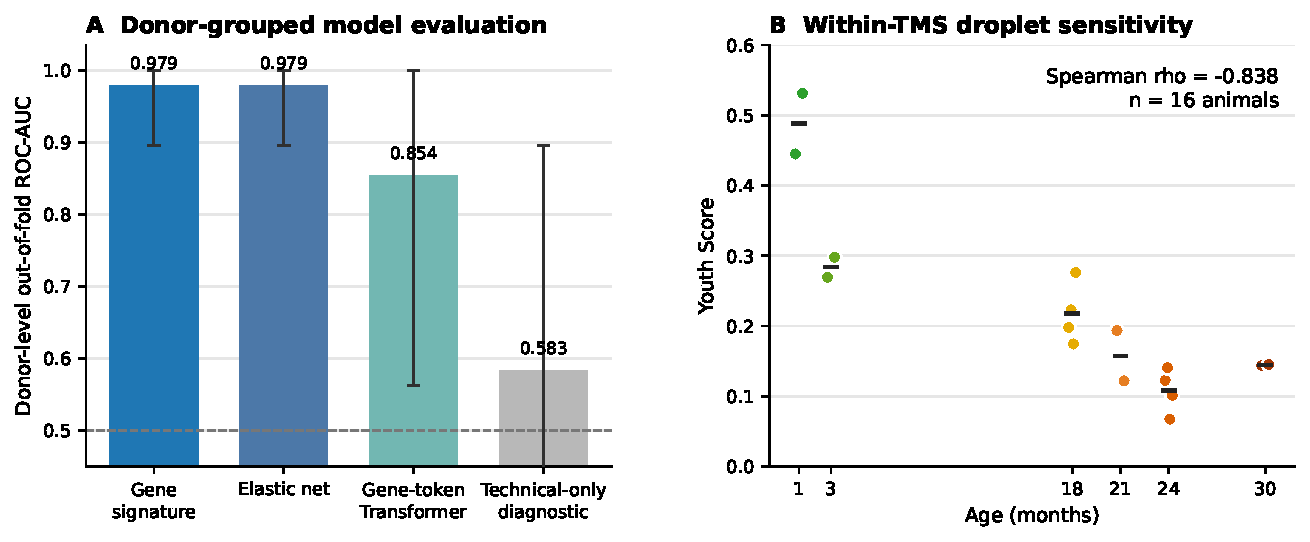
\includegraphics[width=0.43\textwidth,trim=0 0 314.37bp 0,clip]{youth_validation_and_cross_assay.pdf}\\[-1pt]
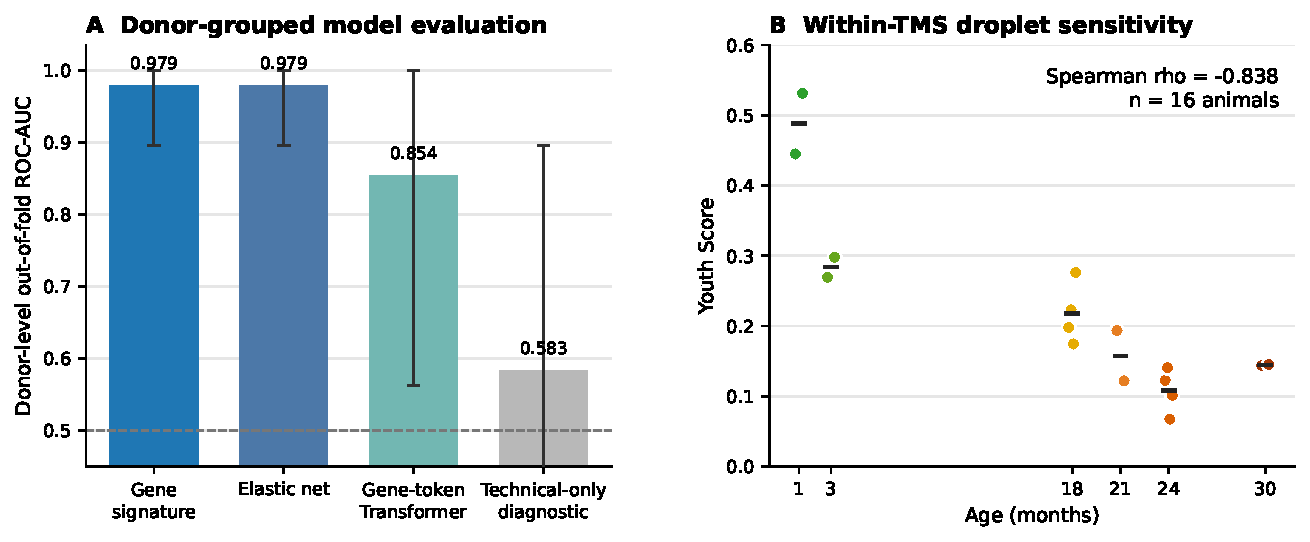
\includegraphics[width=0.43\textwidth,trim=314.37bp 0 0 0,clip]{youth_validation_and_cross_assay.pdf}
\captionof{figure}{Development and within-resource sensitivity of My Youth Score. (A) Donor-level out-of-fold ROC-AUC for candidate models in the cleaned TMS FACS Limb\_Muscle MSC cohort; error bars show donor-bootstrap 95\% intervals. (B) Donor-level scores in TMS droplet Limb\_Muscle MSCs. Points represent animals and horizontal lines represent age-group means. The droplet panel is a cross-assay sensitivity analysis within TMS, not an independent cohort validation.}
\label{fig:youth-validation}
\end{minipage}
\end{strip}

\subsection{Results}

\subsubsection{Internal validation and cross-assay sensitivity}

The gene-signature and elastic-net models achieved the same donor-level out-of-fold ROC-AUC of 0.9792 (Table~\ref{tab:youth-models}). The gene-signature model had the lower Brier score (0.0547 versus 0.0722) and was selected under the prespecified rule. Its PR-AUC was 0.9762, balanced accuracy was 0.9375, F1 score was 0.9231, and its donor-level correlation with age was $\rho=-0.8767$. The gene-token Transformer performed less well in this small donor cohort, whereas the technical-only diagnostic was close to chance (Fig.~\ref{fig:youth-validation}A).

In TMS droplet data, the donor-level Youth Score retained the expected overall age direction ($\rho=-0.8385$, 16 animals; Fig.~\ref{fig:youth-validation}B). Mean scores were 0.4881, 0.2837, 0.2180, 0.1577, 0.1081, and 0.1445 at 1, 3, 18, 21, 24, and 30 months, respectively. The modest increase at 30 months shows that the score is not a strictly monotonic molecular clock.

\begin{strip}
\noindent\begin{minipage}{\textwidth}
\centering
\captionof{table}{Donor-level out-of-fold performance of My Youth candidate models. The technical-only row is a diagnostic rather than a biological candidate.}
\label{tab:youth-models}
\begin{tabular}{lrrrrrr}
\toprule
Model & ROC-AUC & PR-AUC & Balanced accuracy & F1 & Brier & Age Spearman $\rho$ \\
\midrule
Gene signature & 0.9792 & 0.9762 & 0.9375 & 0.9231 & 0.0547 & -0.8767 \\
Elastic net & 0.9792 & 0.9762 & 0.8542 & 0.8333 & 0.0722 & -0.8974 \\
Gene-token Transformer & 0.8542 & 0.9103 & 0.9167 & 0.9091 & 0.1845 & -0.5860 \\
Technical-only diagnostic & 0.5833 & 0.5008 & 0.7292 & 0.7143 & 0.2722 & -0.4126 \\
\bottomrule
\end{tabular}
\end{minipage}
\end{strip}

\subsubsection{Exact-arm evaluation in GSE176206}

In the animal-level four-group summary, mean Youth Scores were 0.5327 for young controls, 0.3658 for young \SOKM, 0.4877 for aged controls, and 0.3440 for aged \SOKM{}. Relative to pooled controls, the \SOKM-minus-control contrast was -0.1669 in young animals and -0.1438 in aged animals.

\newpage
The direction did not depend on pooling the exact controls. In young animals, \SOKM{} differed by -0.1560 from Tg+/Dox- controls and by -0.1779 from Tg-/Dox+ controls. In aged animals, the corresponding differences were -0.1453 and -0.1423. Young controls scored 0.0450 higher than aged controls, whereas the young-minus-aged difference among \SOKM{} animals was 0.0218 and its descriptive interval crossed zero.


\clearpage
\begin{strip}
\noindent\begin{minipage}{\textwidth}
\centering
\begin{minipage}[t]{0.49\textwidth}
\centering
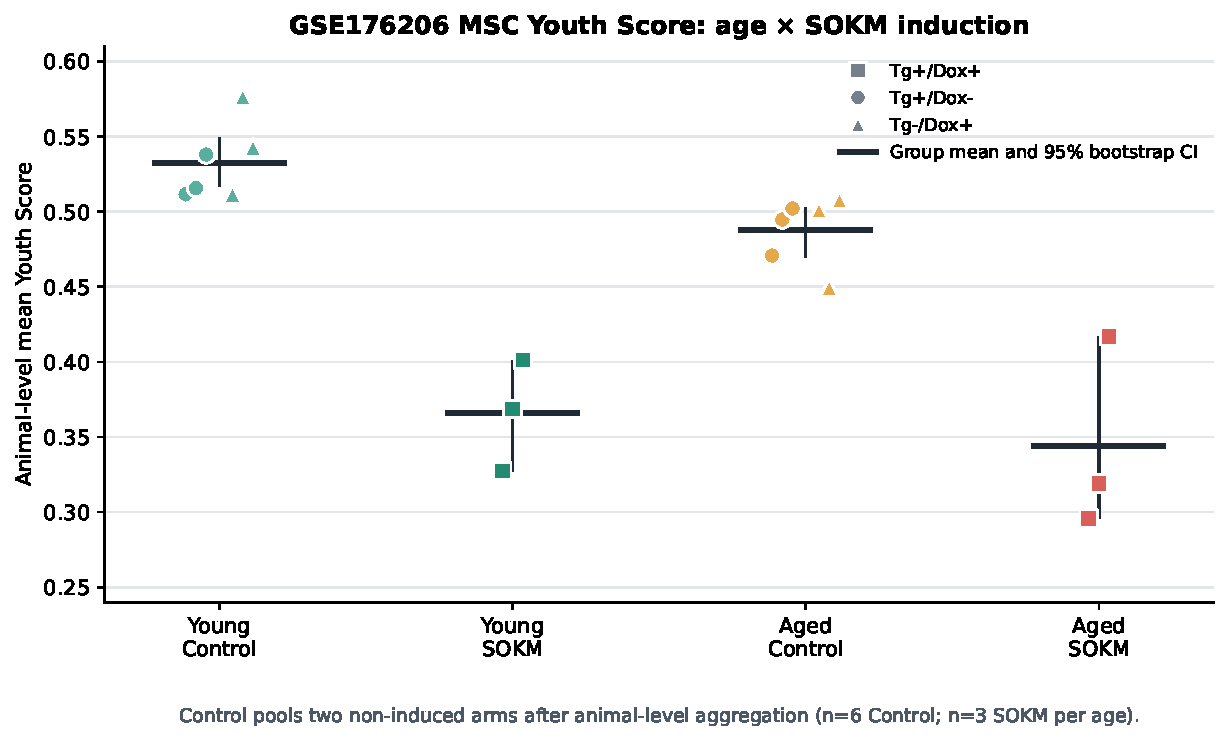
\includegraphics[width=\linewidth]{gse176206_youth_four_group_exact_units.pdf}
\small\textbf{A.} Primary four-group presentation.
\end{minipage}\hfill
\begin{minipage}[t]{0.49\textwidth}
\centering
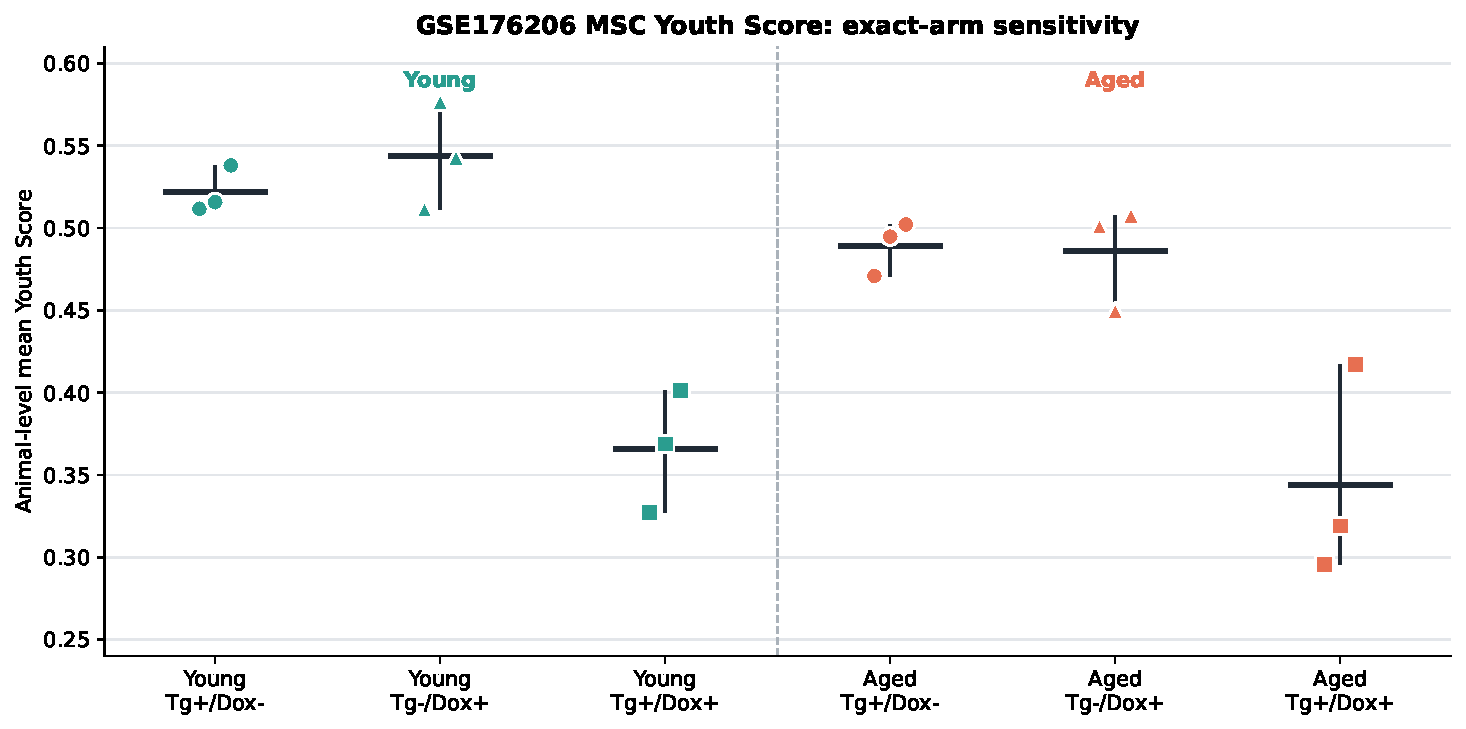
\includegraphics[width=\linewidth]{gse176206_youth_six_exact_arms.pdf}
\small\textbf{B.} Exact-arm sensitivity analysis.
\end{minipage}
\captionof{figure}{My Youth Score in GSE176206. Points represent biological units, not cells. (A) The two control arms were pooled only after animal-level aggregation. (B) Separate control arms preserve the negative \SOKM{} contrast in both age groups. Lower Youth Score means reduced similarity to the young TMS MSC reference; it is not sufficient evidence of accelerated aging.}
\label{fig:youth-gse}
\end{minipage}
\end{strip}

Figure~\ref{fig:youth-gse} shows the animal-level four-group presentation and the exact-arm sensitivity analysis; the corresponding four-group summary is reported in Table~\ref{tab:youth-gse}.


\begin{strip}
\noindent\begin{minipage}{\textwidth}
\centering
\captionof{table}{GSE176206 four-group animal-level Youth Score summary. Controls were pooled only after exact-arm animal aggregation. Intervals are descriptive 95\% animal-bootstrap intervals.}
\label{tab:youth-gse}
\begin{tabular}{llrrl}
\toprule
Age & Analysis group & Animals & Mean Youth Score & 95\% interval \\
\midrule
Young & Control & 6 & 0.5327 & 0.5168 to 0.5492 \\
Young & Tg+/Dox+ \SOKM & 3 & 0.3658 & 0.3273 to 0.4013 \\
Aged & Control & 6 & 0.4877 & 0.4695 to 0.5025 \\
Aged & Tg+/Dox+ \SOKM & 3 & 0.3440 & 0.2958 to 0.4171 \\
\bottomrule
\end{tabular}
\end{minipage}
\end{strip}

\subsection{Module-specific interpretation}

My \YouthScore{} provides a reproducible, reference-dependent age-resemblance coordinate for MSC-like cells. Its strong performance within the TMS FACS domain and the preserved overall age direction in TMS droplet data support this limited interpretation. The compact signature model was preferable to higher-capacity alternatives for the available number of independent animals and reduced the risk of treating abundant cells as biological replication.

The GSE176206 result shows why the word ``Youth'' must remain tied to its training reference. \SOKM-treated animals scored below both exact controls at both ages, but the classifier was trained to distinguish young from old cells within a specific TMS MSC compartment. A treated cell can therefore receive a lower score if its transcriptome shifts away from the reference expression distribution, occupies an intermediate reprogramming state, or becomes unlike both reference classes. The result establishes reduced resemblance to young reference MSCs, not accelerated aging.

\section{MSC Identity Score}

\subsection{Methods}

\subsubsection{Biological definition and gene set}

The \IdentityScore{} was designed as a knowledge-driven composite coordinate of MSC-associated transcription, not as a second age classifier or definitive cell-fate label. Its frozen positive set comprised 11 murine skeletal/stromal-lineage-associated genes curated across bone-marrow MSC and skeletal-progenitor studies: \textit{Cd34, Cd44, Cxcl12, Eng, Itgav, Lepr, Ly6a, Nt5e, Pdgfra, Prrx1}, and \textit{Thy1} \citep{pisterzi2023,greenbaum2013,mo2022,morikawa2009}. Because expression of individual genes is subset- and state-dependent, the panel is a composite reference rather than a set of universal or MSC-exclusive markers. \textit{Vcam1} was excluded because the evidence was insufficiently specific for the mouse limb MSC context. The panel and equal positive weights were frozen before the final GSE176206 comparison without age or treatment labels. Within score construction, known-control labels served only to define the dataset-specific reference for primary-score background matching.

\subsubsection{Primary background-corrected score}

Raw non-negative counts were normalized to 10,000 per cell and log transformed as in the Youth analysis. The primary score corrected mean observed-panel expression with 100 expression-matched background sets. Mean expression in 3,694 known-animal control cells defined 24 bins; for each identity gene and set, one eligible gene was sampled from its bin. The eligible pool excluded all included genes in the complete frozen reprogramming-module resource and predefined technical-noise genes. Sampling used seed 20260729:
\begin{equation}
I_c^{\mathrm{primary}}=
\frac{1}{|G_I|}\sum_{g\in G_I}x_{cg}
-\frac{1}{100}\sum_{b=1}^{100}
\left(\frac{1}{|B_b|}\sum_{g\in B_b}x_{cg}\right).
\end{equation}

\subsubsection{Rank-based sensitivity score}

As a sensitivity analysis, expressed genes were converted to within-cell percentiles; an undetected identity gene received zero. The rank-based score was
\begin{equation}
I_c^{\mathrm{rank}}=\frac{1}{11}\sum_{g\in G_I}r_{cg}.
\end{equation}
The two scores capture complementary properties of the frozen panel---expression-matched enrichment and within-cell percentile prominence---on different scales. Neither is a calibrated probability of MSC identity; raw magnitudes were not compared.

\subsubsection{Quality control and aggregation}

Input feature matrices had to contain at least 70\% of the 11 frozen symbols, a dataset-level mapping rule rather than a per-cell detection threshold. GSE176206 contained all 11 and produced no missing cell scores. The prespecified analysis used the same 18 age-by-exact-arm animal units as Youth. The median cell score was the primary unit summary; mean and 95th percentile were supporting outputs. Arms were unpaired, and unknown-animal or negative-control cells were excluded.

\subsection{Results}

The pipeline scored all 20,661 cells; 18,686 entered the formal animal-level analysis, and all prespecified checks passed. The prespecified primary panel score was comparator dependent. Aged condition medians were 0.1482 (\SOKM), 0.2762 (Tg+/Dox-), and 0.1457 (Tg-/Dox+); young medians were 0.1511, 0.2846, and 0.1685, respectively. Thus, the \SOKM{} median was lower than Tg+/Dox- but close to Tg-/Dox+, particularly in aged animals.

The rank-based sensitivity metric showed more consistent descriptive arm separation. Aged condition medians were 0.3104 (\SOKM), 0.4831 (Tg+/Dox-), and 0.4845 (Tg-/Dox+); young medians were 0.3328, 0.4824, and 0.4967, respectively.

The exact-arm condition summaries and animal-level distributions are shown in Table~\ref{tab:identity} and Fig.~\ref{fig:identity}, respectively.

\begin{strip}
\noindent\begin{minipage}{\textwidth}
\centering
\captionof{table}{GSE176206 Identity panel scores, summarized as the median of three animal-level medians per exact arm. Primary and rank-based scores occupy different scales.}
\label{tab:identity}
\small
\begin{tabular}{llrr}
\toprule
Age & Exact arm & Primary Identity Score & Rank-based Identity Score \\
\midrule
Young & Tg+/Dox+ \SOKM & 0.1511 & 0.3328 \\
Young & Tg+/Dox- control & 0.2846 & 0.4824 \\
Young & Tg-/Dox+ control & 0.1685 & 0.4967 \\
Aged & Tg+/Dox+ \SOKM & 0.1482 & 0.3104 \\
Aged & Tg+/Dox- control & 0.2762 & 0.4831 \\
Aged & Tg-/Dox+ control & 0.1457 & 0.4845 \\
\bottomrule
\end{tabular}
\end{minipage}
\end{strip}


\subsection{Module-specific interpretation}

The animal-level distributions underlying the condition summaries are shown in Fig.~\ref{fig:identity}. The \IdentityScore{} reports the prominence of a predefined MSC-associated composite panel and does not adjudicate lineage identity. Because the panel itself was curated without age or treatment labels, it contextualizes Youth without altering that calculation. The rank-based analysis placed \SOKM{} units below both control arms at both ages within this cohort; because ranks are relative, this does not establish absolute marker loss or loss of MSC identity. Comparator dependence of the primary score also prevents a universal identity-loss claim.

Rank scoring measures the within-transcriptome position of panel genes, whereas background correction measures enrichment relative to expression-matched genes; changes in global composition or detectability can therefore make them diverge. Neither score establishes reduced differentiation capacity or an alternative lineage without orthogonal evidence.

\begin{strip}
\noindent\begin{minipage}{\textwidth}
\centering
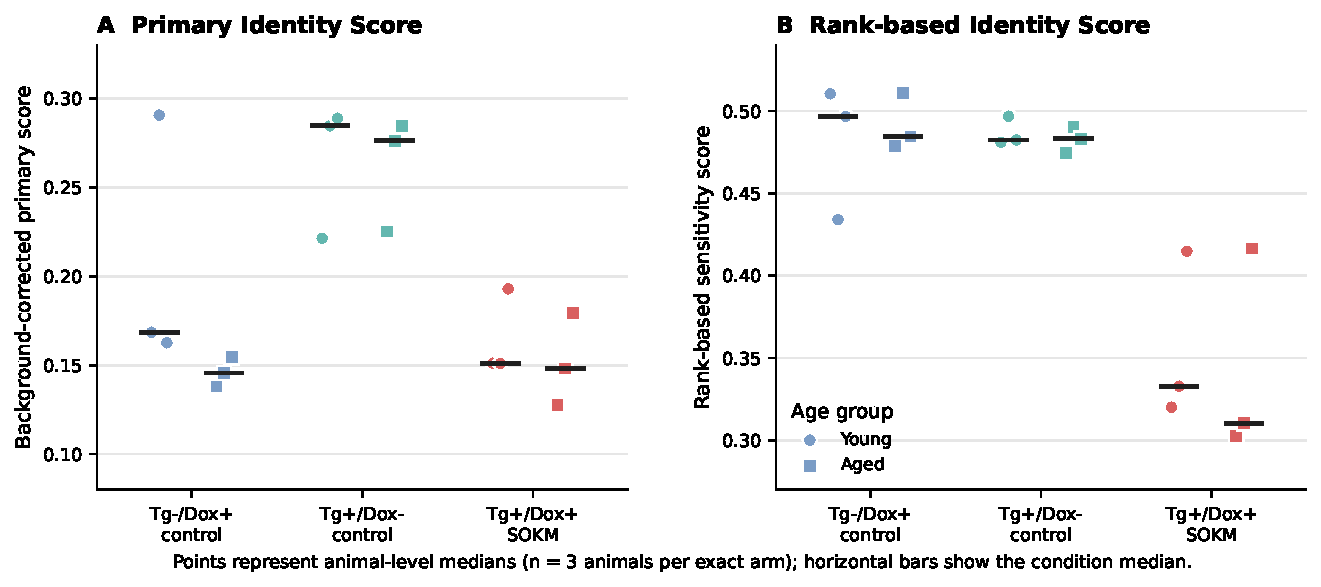
\includegraphics[width=0.85\textwidth]{identity_exact_arm_scores.pdf}
\captionof{figure}{MSC Identity Scores across the GSE176206 exact arms. Each point is the median cell score for one animal; short horizontal bars show the condition median. Circles denote young animals and squares denote aged animals. The rank-based condition median was lower under \SOKM{} than under both controls at both ages, whereas the background-corrected primary score was comparator dependent. Panels use separate scales.}
\label{fig:identity}
\end{minipage}
\end{strip}

\clearpage
\begin{strip}
\noindent\begin{minipage}{\textwidth}
\centering
\begin{tikzpicture}[
  node distance=11mm and 18mm,
  box/.style={rounded corners=2pt, draw=black!40, very thick, align=center, minimum height=14mm, text width=47mm, fill=SoftGray},
  youth/.style={box, draw=YouthBlue, fill=YouthBlue!8},
  identity/.style={box, draw=IdentityTeal, fill=IdentityTeal!8},
  result/.style={box, draw=SOKMRed, fill=SOKMRed!7, text width=54mm},
  arrow/.style={-{Latex[length=2.2mm]}, thick, draw=black!65}
]
\node[youth] (youth) {\textbf{Youth axis}\\Similarity to the young TMS FACS Limb\_Muscle MSC reference};
\node[identity, right=of youth] (identity) {\textbf{Identity axis}\\Frozen 11-gene MSC-associated composite-panel coordinate};
\node[result, below=of $(youth)!0.5!(identity)$] (joint) {\textbf{Two reported observations}\\Departure from the young MSC reference; change on the frozen Identity-panel coordinate};
\node[box, below left=9mm and -5mm of joint, text width=55mm] (notage) {\textbf{Not established}\\Accelerated aging, functional rejuvenation, or loss of potency};
\node[box, below right=9mm and -5mm of joint, text width=55mm] (notmath) {\textbf{No mathematical correction}\\Identity remains an independent explanatory coordinate};
\draw[arrow] (youth) -- (joint);
\draw[arrow] (identity) -- (joint);
\draw[arrow] (joint) -- (notage);
\draw[arrow] (joint) -- (notmath);
\end{tikzpicture}
\captionof{figure}{Reference-aware interpretation of the two modules. Youth and Identity describe different properties of a cell state and are combined only at the interpretive level. A lower Youth Score means reduced resemblance to the young reference, not accelerated aging. Identity quantifies a composite panel coordinate and remains an independent axis, not a correction term.}
\label{fig:framework}
\end{minipage}
\end{strip}

\section{Integrated Interpretation}

Figure~\ref{fig:framework} summarizes this reference-aware interpretation and the strict separation between the two axes. The frozen Youth model reported lower similarity to young TMS MSCs after \SOKM{} exposure. Independently, the Identity module showed treatment-associated differences on the predefined composite panel: the rank-based sensitivity score was lower across both comparators, whereas the prespecified primary score was comparator dependent. These separately reported observations are compatible with \SOKM{} states that differ from the young MSC reference while occupying a different position on the identity-panel coordinate; they do not establish accelerated aging.

Youth and Identity remain separate axes. Identity was not used to rescale or correct Youth. A low Identity Score does not change the computed Youth Score, but it cautions against interpreting that value as rejuvenation outside the young-MSC reference context. For cross-module integration, native animal-level outputs should be joined by shared biological-unit identifiers and retained as separate named outputs with their native scales and quality-control fields; missing outputs should not be imputed, and the axes should not be collapsed into an unvalidated scalar.


\subsection{Limitations}

Several limitations constrain inference. First, the Youth model learned a binary 3-month-versus-18/24-month contrast from 14 animals and is therefore not a continuous aging clock. Second, the TMS droplet analysis is confounded by age, sex, donor composition, and assay technology; it supports cross-assay sensitivity rather than independent cohort validation. Third, GSE176206 contained three animals per age-by-exact-arm stratum and highly unequal cell counts among animals. Animal aggregation prevents pseudoreplication but cannot overcome the small biological sample size, and the bootstrap intervals are descriptive.

Fourth, neither module directly measures cellular function. Youth cannot establish rejuvenation or accelerated aging, and Identity cannot establish potency or lineage fidelity. Fifth, the Identity module uses a compact literature-curated composite panel whose genes are subset- and state-dependent; other tissues, species, or MSC definitions may require a different marker contract. Its background model was estimated within the analyzed dataset and may retain cohort dependence. Finally, these analyses do not define a validated ``safe zone,'' establish oncogenic safety, or prove causal relations among Youth, Identity, and Risk.

The defensible conclusion is therefore narrow: in GSE176206 cells annotated as muscle-derived MSCs, \SOKM{} treatment was associated with decreased resemblance to the young TMS MSC reference. The rank-based Identity sensitivity score was lower in \SOKM{} than in both exact control arms at both ages, whereas the prespecified primary score was comparator dependent. The two-axis framework permits these statements without redefining either as proof of biological aging, rejuvenation, lineage conversion, or safety.


\bibliographystyle{unsrtnat}
\bibliography{references}

\end{document}
